\chapter{Data quality challenge}

This chapter details one of the main challenges Alkemics faces, and how we tackled it. 
After presenting what is data-quality and why it matters, we will present how we built a suggestion workflow that helps our users to detect errors, and provides potential corrections. Finally we will detail what tools we built to monitor and control quality.

The detail of machine learning algorithms used to provide predictions will be detailed in next chapter.

\section{Stakes}

Reliable, up-to-date, accessible, tracable, products data is one of the core value proposition of Alkemics services for retailers.

To provide this service, Alkemics teams have put a lot of effort in building:

\begin{itemize}
	\item bridges between data-models: Mondelez data-model is not the same as Pepsi, or Auchan's one. Alkemics data-model aims at generalizing all others and have the ability to translate any product data in other data-models.
	\item bridge between data-stores: APIs and interfaces to easily import or export data in several formats.
	\item bridges between people: ability to communicate easily about products through the platform
\end{itemize} 

Ultimately, data is owned and provided by manufacturers, and then shared with retailers.

\subsection{What is data-quality}

Data quality can be evaluated through:
\begin{itemize}
\item completeness: the product page has sufficient details about the product.
	\begin{itemize}
		\item regulatory fields: for instance if your product contains alcohol you must provide the alcohol concentration.
		\item retailer specific fields: some retailer set their own requirements to sell on their platforms
	\end{itemize}
\item accuracy: the provided data is accurate, there is no error.
\end{itemize}


\subsection{Why it matters}

\textbf{Data quality is a major issue to retailers}

\begin{itemize}
\item Regulatory: internet retailers have the obligation to provide some specific informations on the products. If they don't they can be heavily fined. Fields as 
\item Marketing: display detailed information about products to customers. Would you buy products with no description?
\item Search: to correctly index products you need data, for instance how will your customer find strawberry icecream is flavors fields are not well filled. Well indexed products is key to performant search engine on web plateforms.
\item Logistics: weight, size, number of units etc. These fields allow retailers to correctly handle logistics.
\end{itemize}

The growing part of online groceries.
The rise of Amazon is a direct threat to all retailers. One of Amazon's advantages is its huge ability to handle data-flows.

\subsection{Why is the data of poor quality}

Some of the reasons are:

\begin{itemize}
\item many actors have to communicate: +50k manufacturers, dozens of retailers. Each manufacturer has to send its data to each retailer sending its products => hundreds of thousands of connections
\item no fully accepted data-model standard. Even though GDSN standard is dominant, not all companies are compliant with it.
\item actors interested in data-quality (primarly retailers), rely on actors for which it is less crucial (makers)
\item products data identification numbers (EAN) frequently change
\end{itemize}

\subsection{What can we do about data-quality}

Given a product, we want to predict several of its attributes given some basic fields that are nearly always filled.
The predicted fields for now are:
\begin{itemize}
	\item hazard pictograms (inflammable, corrosive etc ...)
	\item labels (organic, made in France, eco-packaging etc...)
	\item category in Alkemics data-model (Processed meat, Cereal, baked product etc...)
	\item allergens (walnut, lactose, sulfite etc ...)
\end{itemize}

After these predictions are made, we want to evaluate it against products attributes to warn the manufacturers if we think that some of its data is incomplete or innacurate.

\subsection{What are our constraints}
\begin{itemize}
\item we cannot unilaterally change manufacturers data: they own their data
\item we must garanty a high degree of confidence on suggestions we make, especially at the begining, otherwise manufacturers won't trust and use our suggestions
\item predictions must be made regularly (product data continuously evolve)
\item predictions must adapt to data-model changes
\item our predictive models hade to perform well on datasets of poor data-quality (some fields are nearly never filled)
\item we must be able to monitor closely how well our models perform, and how well perceived are our suggestions 
\end{itemize}


\pagebreak
\section{Suggestion Workflow to improve data-quality}


This part aims at presenting the workflow we use to provide attribute suggestions on product pages‡ to our users.

\begin{figure}[H]
\centering
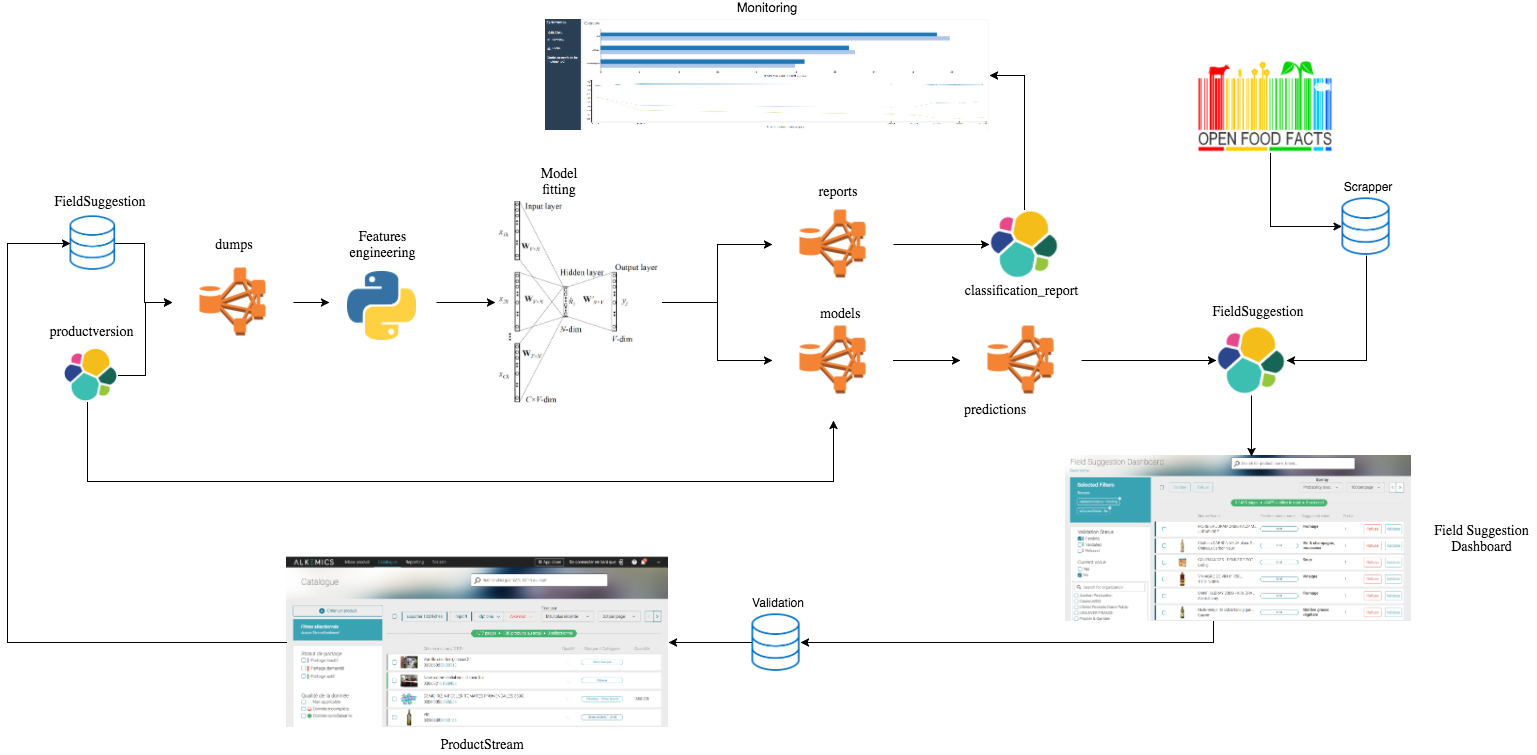
\includegraphics[scale=0.30]{./images/workflow/fieldsuggestion-workflow.png}
\caption{Suggestion workflow overview.}
\end{figure}

\subsubsection{Workflow steps}
\begin{enumerate}
	\item extraction of some attributes (name, description, composition) from products
	\item feature engineering (NLP preprocessing)
	\item training on labeled products (fasttext model) and report
	\item prediction (on all products)
	\item indexation as suggestion
	\begin{itemize}
		\item from machine learning suggestions
		\item from scrapped websites (major one: OpenFoodFacts)
	\end{itemize}
	\item suggestion validation by Alkemics
	\item display of validated suggestions to users in product pages
	\item suggestion acceptation by users
\end{enumerate}


% For product 1198365 / 07622300788063: https://stream.alkemics.com/#/catalog/07622300788063


\subsection{Feature and labels extraction}

From product database.
From validation database: suggestion validated by Alkemics, not yet accepted/refused by client. -> ability to bootstrap and improve models. 

The idea is to get gather enough information from products (-> more fields), but on fields with sufficient completion (-> less fields).

\begin{lstlisting}[language=json]
{
    "brand": "Grany",
    "namePublicLong": "Grany Coeur Fondant Gout Chocolat Noisettes 120g",
    "nameLegal": "BARRE CEREALIERE FOURREE AU CHOCOLAT ET A LA NOISETTE.",
    "composition": "Ingrédients: Céréales 31,5% (farine de RIZ 9,1%, farine de BLÉ 5,6%, grains de maïs 4,7%, flocons de BLÉ 4,5%, flocons d'AVOINE 4,5%, flocons d'ORGE 2,5%, farine de BLÉ malté 0,6%), sirop de glucose-fructose, sucre, huile de coprah, LAIT écrémé en poudre, huile de palme, chocolat 5% (sucre, pâte de cacao), pâte de NOISETTES 5%, cacao maigre en poudre, humectant (glycérol), sel, gluten (de BLÉ), dextrose, émulsifiant (lécithine de tournesol), malt d'ORGE, arôme (NOISETTES), ARACHIDE. PEUT CONTENIR SOJA, AUTRES FRUITS À COQUE.',
    "description": "Grany au cœur Chocolat au Lait et aux Noisettes, le plaisir brut des céréales associées au fondant du chocolat au lait !",
    "advices": "",
    "healthAllegations": ""
}
\end{lstlisting}

\subsection{Feature engineering}

Transforming these features in a relevant input format for our models. 
The models we use will be detailed in next chapter. Theses models accept similar input as famous NLP models such skip-gram or c-bow.

This is classic NLP preprocessing.

\begin{enumerate}
	\item concatenated fields as string
	\item normalize text (encoding -> ascii)
	\item tokenize
	\item for each token:
	\begin{itemize}
		\item lower
		\item remove eventual html tags
		\item filter stopwords and punctuation
		\item remove digits
		\item stem
	\end{itemize}
	\item concatenate tokens
\end{enumerate}

\begin{lstlisting}[language=json]
"grany cur chocolat lait noiset plais brut cereal associe fond chocolat lait grany barr cerealier fourre chocolat noiset grany coeur fond gout chocolat noiset ingredient cereal farin riz farin ble grain flocon ble flocon avoin flocon orge farin ble malt sirop glucos fructos sucr huil coprah lait ecrem poudr huil palm chocolat sucr pat cacao pat noiset cacao maigr poudr humect glycerol sel gluten ble dextros emulsifi lecithin tournesol malt orge arom noiset arachid conten soj autr fruit coqu"
\end{lstlisting}

\subsection{Training stage}

Training stage includes:
\begin{itemize}
	\item labeled-set preprocessing
	\item split train/test:
	\item train on train, predict on test
	\item compute scores reports on both train-set and test-set
	\item compute global/local precision curves
	\item save model for further use
	\item index reports for monitoring
\end{itemize}


Multiclass labeled-set preprocessing: every sample has one and only one label
- filter labeled items
- remove classes with not enough occurences

Multilabel labeled-set preprocessing: samples can have 0->n labels
- a sample can be considered even though it has no label
- remove classes with not enough occurences from label lists

\subsection{Predict stage}
Predict stage includes: 
\begin{itemize}
	\item extracting all product features (label AND non-labeled)
	\item compute prediction scores
	\item enrich prediction with recall/precision estimations based on prediction score and local precision/recall curves computed during training-stage
	\item save all predictions with scores > 0.05
\end{itemize}

\subsection{Machine learning suggestion indexation with scrapped information}

Suggestions from machine learning, are merged with suggestions issued from web-scrapping.
Those suggestions are indexed together to provide a global score (number of concordant sources) to suggestions.


Annexe:
\begin{lstlisting}[language=json]
{
    "_type": "fieldsuggestion",
    "extended_attributes": {
        "precision_group": 0.91489,
        "features": "grany cur chocolat lait noiset plais brut cereal...",
        "probability": 0.87393,
        "recall_group": 0.55128
    },
    "entity_type": "carrefour_drive",
    "field": {
        "status": 0,
        "fieldmetadata_name": "hasnotableingredients",
        "fieldmetadata_id": 107,
        "is_current_value": 0,
        "field_id": 59,
        "field_name": "arachide"
    },
    "id": "1198365_107_59",
    "metadata": {
        "global_score": 4,
        "product_id": 142292,
        "media": "https://smedia.alkemics.com/product/142292/...",
        "brand": "Grany",
        "contentowner": {
            "id": 356,
            "name": "Mondelez International"
        },
        "sources": [
            "carrefour_drive",
            "intermarche",
            "openfoodfacts",
            "ml"
        ],
        "gtin": "07622300788063",
        "productversion_id": 1198365,
        "name": "Grany Coeur Fondant Gout Chocolat Noisettes 120g"
    }
}
\end{lstlisting}


\subsection{Validation (or refusal) from Alkemics}
Since we must reach a high degree of confidence in our predictions, and since we do not yet have history about how well we perform, each suggestion is manually validated. (Suggestions issued from 2 or more sources are automatically validated).

\begin{figure}[H]
\centering
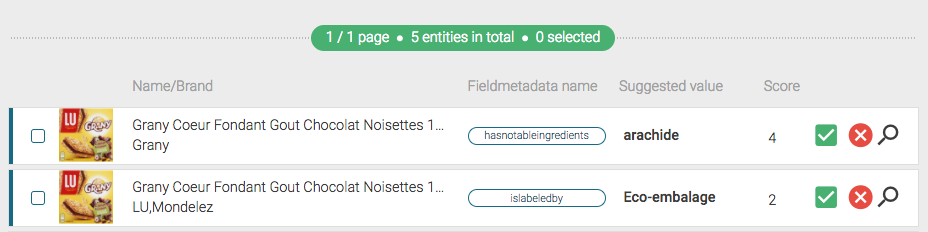
\includegraphics[scale=0.50]{./images/workflow/validation-suggestion.png}
\caption{Suggestion validation by Alkemics.}
\end{figure}


\subsection{Suggestion display to users in product pages, and acceptation (or dismissal) from manufacturer}

\begin{figure}[H]
\centering
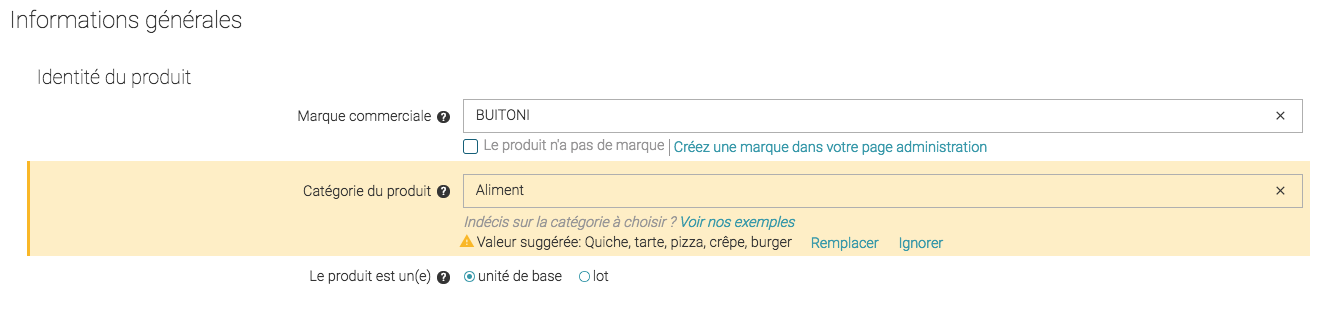
\includegraphics[scale=0.35]{./images/workflow/stream-suggestion-3.png}
\caption{Suggestion acceptation by user.}
\end{figure}





\pagebreak
\section{Monitoring}
Given the complexity of the workflow, and quality expected by clients, we have to closely monitor some metrics:
\begin{itemize}
	\item is there an evolution of classes distribution
	\item how our scores behave at training stage
	\item whether our predictions get rejected at validation stage
	\item do our validated suggestion get dismissed by user at acceptation stage
\end{itemize}

\subsection{Performance metrics definition}

Evaluation metrics should take into account the class imbalance between churners and non-churners. A greater cost should be associated with false negatives than with false positives: misidentify a potential churner costs far more to a company than identifying a non-churner as churner. Moreover, we are more interested in perfectly identifying those customers who are most likely to churn than perfectly identifying \textit{all} the potential churners.

\subsubsection*{Binary classification metrics}

As we are in a binary classification problem, several metrics can be used to assess the performance of the models.

Lets define some naming/metrics used in the following:

{\ttfamily
\begin{table}[H]
    \centering
    \begin{tabular}{ll}
        \toprule
        $TP / FP$          &    $true/false\ positives$ \\
        $TN / FN$       &    $true/false\ negatives$  \\
        $P$       &    $TP+FN$ \\
        $N$    &    $TN + FP$ \\
        $recall$      &    ${TP} / {P}$ \\
        $precision$        &   ${TP} / {(TP+FP)}$ \\
        $Yrate$      &    $(TP+FP) / {(P+N)}$ \\
        $FPrate$      &    ${FP} / {N}$ \\
        \bottomrule
    \end{tabular}
\caption{some metrics}
\end{table}
}

Precision, recall and accuracy are often used to measure the classification quality of binary classifiers.

In customer churn prediction, the misclassification of a churner may result in the loss of the customer but the misclassification of a non-churner may result in some extra marketing cost.  Because the former is more costly than the latter, recall is a more important measure than precision \cite{VdP05}.
While precision and recall measure how accurate the methods can identify the observations in a single class, the AUC measures how well the methods discriminate the two classes.

Precision measures that fraction of examples classified as churner that are truly churner.

Recall measures the fraction of well classified churners.

\subsubsection{note} % (fold)
\label{ssub:note_1}
The problem of churn differs from classical classification/prediction setups, notably in the objectives to optimize on. Although having a good recall, for instance, is important (we want as many churners well classified as possible), one should really take into account the \textit{business application}: a typical use of a churn prediction model is to target potential future churners and to launch a marketing campaign to retain them. In such cases, we are willing to tolerate greater overall error, in return for better identifying the most likely future churners for further attention.

Contacting a large proportion of the customers is expensive: one wants to maximize the number of potential churners reached while minimizing the total number of contacted customers. Metrics such as \textit{lift} (\ref{sub:lift}) express very well this business application constraint.

% subsubsection note (end)

\subsection{F-score} % (fold)
\label{sub:fbeta_score}

The $F_1$ is a measure of a classifier accuracy, computed as the harmonic mean of precision and recall: $$F_1= 2. \frac{precision.recall}{precision+recall}$$\tabularnewline
This definition assign the same weight to precision and recall but in our case, recall is more valuable than precision: we want all the churners to be correctly classified and type I error has less monetary impact (people may be targeted for a marketing campaign even if they weren't about to churn).

To handle these constraints, the $F_\beta-score$ is adapted: in consists in the \textit{weighted} harmonic mean of recall and precision, assigning $\beta$ times as much importance to recall as precision: $$F_\beta = (1+\beta^2) \frac{precision.recall}{\beta^2.precision+recall}$$

% subsection fbeta_score (end)

\subsection{Calibration plot} % (fold)
\label{sub:calibration_plot}

When dealing with probabilistic classifiers, one of the signs that a suitable classification model has been found is also that predicted probabilities (scores) are well calibrated, that is that a fraction of about $p$ of events with predicted probability $p$ actually occurs. Calibration plot is a method that shows us how well the classifier is calibrated \cite{VC06}: $$x = true\ probability,\ y=predicted\ probability$$

True probabilities are calculated for (sub)sets of examples with the same predicted score $P(y=1|X) \in [c-\delta, c+\delta]$: $$ p_{true}^c = \frac{P_{sub}^c}{P_{sub}^c + N_{sub}^c}$$ with $P_{sub}^c, N_{sub}^c$ being the proportion on positives and negative examples in a given subset with predicted probabilities $[c-\delta, c+\delta]$. The calibration plot of a perfectly calibrated classifier will be a diagonal.


\subsubsection*{Multiclass-multilabel classification metrics}

\subsubsection*{Pursuived objectives: precision/recall }


\subsection{Workflow graph}

\subsection{Bootstrap}
